% Source for the figure of SPlusTree (sec. 6.3): an S+ tree of B = 4 keys a
% node on 16 sorted items, the root over the four leaves (the items
% themselves), and the search of v = 26, which counts 2 keys smaller than v
% in the root and 2 in the leaf 2, i.e., the place 2 B + 2 = 10. Build:
% make figures (in ../build).
\documentclass[border=4pt]{standalone}
\usepackage[T1]{fontenc}
\usepackage{newpxtext,newpxmath}
\usepackage[varqu,varl,scaled=0.95]{zi4}
\usepackage{tikz}
% tikz-ads.tex: the TikZ styles shared by the figures of the memory of the
% manual, \input by each standalone figure: a cell of a vector (cell), the
% cell that an operation touches (touched), a free cell (free), a node of a
% linked structure (node), the labels of indices (index) and of variables
% (var), a pointer (ptr), and \cells and \indices to draw a row of cells.
\usetikzlibrary{arrows.meta,positioning,calc,fit,shapes.multipart}
\definecolor{adsTouched}{RGB}{214,196,236}
\definecolor{adsFree}{RGB}{236,236,236}
\tikzset{
  ads/.style={>={Stealth[length=2mm]},font=\small,
              every node/.append style={inner sep=0pt}},
  cell/.style={draw,minimum width=7mm,minimum height=7mm,
               font=\small\ttfamily,outer sep=0pt},
  touched/.style={cell,fill=adsTouched},
  free/.style={cell,fill=adsFree,text=black!45},
  node/.style={draw,rounded corners=1pt,minimum width=8mm,
               minimum height=6mm,font=\small\ttfamily},
  index/.style={font=\scriptsize\ttfamily,text=black!60},
  var/.style={font=\small\itshape},
  ptr/.style={->,thick}
}
% \cells{name}{x,y}{list}: a row of cells, the first at (x,y), named
% name-0, name-1, ...; each item is text/style, the style one of cell,
% touched and free (e.g., {a/cell,e/touched,/free})
\newcommand{\cells}[3]{%
  \foreach \v/\s [count=\i from 0] in {#3}
    \node[\s] (#1-\i) at ($(#2)+(\i*7mm,0)$) {\v};}
% \indices{name}{n}: the indices 0 .. n-1 under the cells of name
\newcommand{\indices}[2]{%
  \foreach \i in {0,...,\numexpr#2-1\relax}
    \node[index,below=1.2mm of #1-\i] {\i};}

\begin{document}
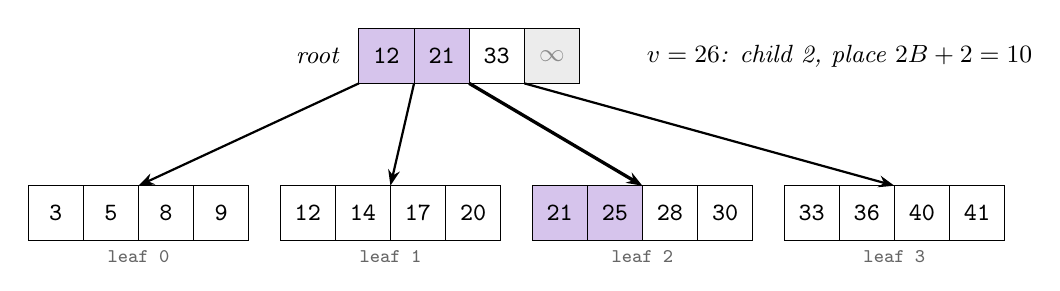
\begin{tikzpicture}[ads]
  \node[var,anchor=east] at (36mm,0) {root};
  \cells{r}{42mm,0}{12/touched,21/touched,33/cell,$\infty$/free}
  \cells{a}{0,-20mm}{3/cell,5/cell,8/cell,9/cell}
  \cells{b}{32mm,-20mm}{12/cell,14/cell,17/cell,20/cell}
  \cells{c}{64mm,-20mm}{21/touched,25/touched,28/cell,30/cell}
  \cells{d}{96mm,-20mm}{33/cell,36/cell,40/cell,41/cell}
  \draw[ptr] (r-0.south west) -- (a-1.north east);
  \draw[ptr] (r-0.south east) -- (b-1.north east);
  \draw[ptr,very thick] (r-1.south east) -- (c-1.north east);
  \draw[ptr] (r-2.south east) -- (d-1.north east);
  \foreach \n/\k in {a/0,b/1,c/2,d/3}
    \node[index,below=1.2mm of \n-1.south east] {leaf \k};
  \node[var,anchor=west] at (75mm,0) {$v = 26$: child 2, place $2 B + 2 = 10$};
\end{tikzpicture}
\end{document}
